\chapter{Extending Reinforcement Learning in Diffusion Models}

The code repository \href{https://github.com/alcazar90/ddpo-celebahq}{https://github.com/alcazar90/ddpo-celebahq}.

\section{Introduction}

\textbf{TODO:} Introducir los modelos de difusión y luego la intersección de
estos con reinforcement learning. \\

Reinforcement learning has shown the capacity to orchestrate or align highly complex generative models, which often proves intractable using supervised learning matching distribution objective. Constructing agents based on generative models can be seen as an user-model interface, an intriguing line of exploration from the perspective of human-computer interaction (HCI). While reinforcement learning is not a cheap or intuitive approach, it offers flexibility and simplicity by optimizing a reward. Regarding the cost of sampling, highly capable generative models such as LLMs and diffusion models have fostered research efforts to reduce inference times for sample generation (inference as a first citizen). These advances make it more appealing to construct agents atop these models. \\

In this work, we propose several extensions to the formulation of the diffusion process as a sequential decision-making process, specifically regarding how to exploit the information from the intermediate state rewards rather than only using the final trajectory outcome. Based on the \textit{insights} of the reward signal behavior in sample generation, we propose methods based on the challenge classifier guidance techniques from the diffusion model literature. Moreover, we explore the use of baseline functions, a technique known to reduce the variance of the gradient estimator when using Monte Carlo estimation \cite{mohamed2020monte}, without introducing bias into the estimator. We compare the implementation of these extensions to the DDPO algorithm \cite{black2023training} on which our formulation is based, on the same \textit{downstream tasks} used in this work, such as JPEG compressibility, JPEG incompressibility, and aesthetic quality as proposed in \cite{black2023training}. \\

Our contributions extend the existing framework of the diffusion process by exploiting the informative intermediate state rewards rather than solely relying on the final trajectory outcome. We analyze the reward signal dynamics throughout the denoising process using a collection of sample trajectories from the \textit{google/ddpm-celebahq-256} model. Additionally, we propose extended reward functions that incorporate further information beyond the final sample, alongside the introduction of baseline functions during RL training. We compare the implementation of these extensions with the DDPO algorithm, highlighting the advantages of our framework in downstream tasks such as JPEG compressibility, JPEG incompressibility, and aesthetic quality assessment.

\section{Related Work}

\textbf{TODO:} Esta sección tiene que ser escrita muy en modo paper Neurips
para reciclar lo máximo posible. Explicar el trabajo de Black y otros. \\


Introducir qué es Reinforcement Learning with Human Feedback. Vincular con el paper de Ouyang en modelos de lenguaje: Training language models to follow instructions with human feedback. Ver tambien el substack de Nathan Lambert (https://www.interconnects.ai/p/specifying-objectives-in-rlhf). 

Papers relevantes para establecer relación entre modelos de difusión y RL.

\begin{itemize}
    \item Training Diffusion Models with Reinforcement Learning (Black 2023)
    \item Aligning Text-to-Image Models using Human Feedback (Lee 2023). Interesting discussion about how to train the reward function, this work provides pseudo-code with the steps used for training. However, the apporach purposed in this work is off-line and doesn't generate samples to update the model using a policy optimization algorithm like DDPO.
    \item Trust Region Policy Optimization \& Proximal Policy Optimization Algorithms (Schulman 2015 and 2017). The former work extend a theoretical lower bound that works for policy update, original present for the case of mixture policies (something between $\pi_{old}$ and $\pi`$), and now adapted to stochastic policies. They introduce a distance measure between policies: total variation divergence. 
\end{itemize}

\section{Background: Diffusion Model as Sequential Decision-making Process}

Several works postulate probabilistic models as MDPs...

% Diffusion Model as MDP
\begin{figure}[ht]
  \centering
  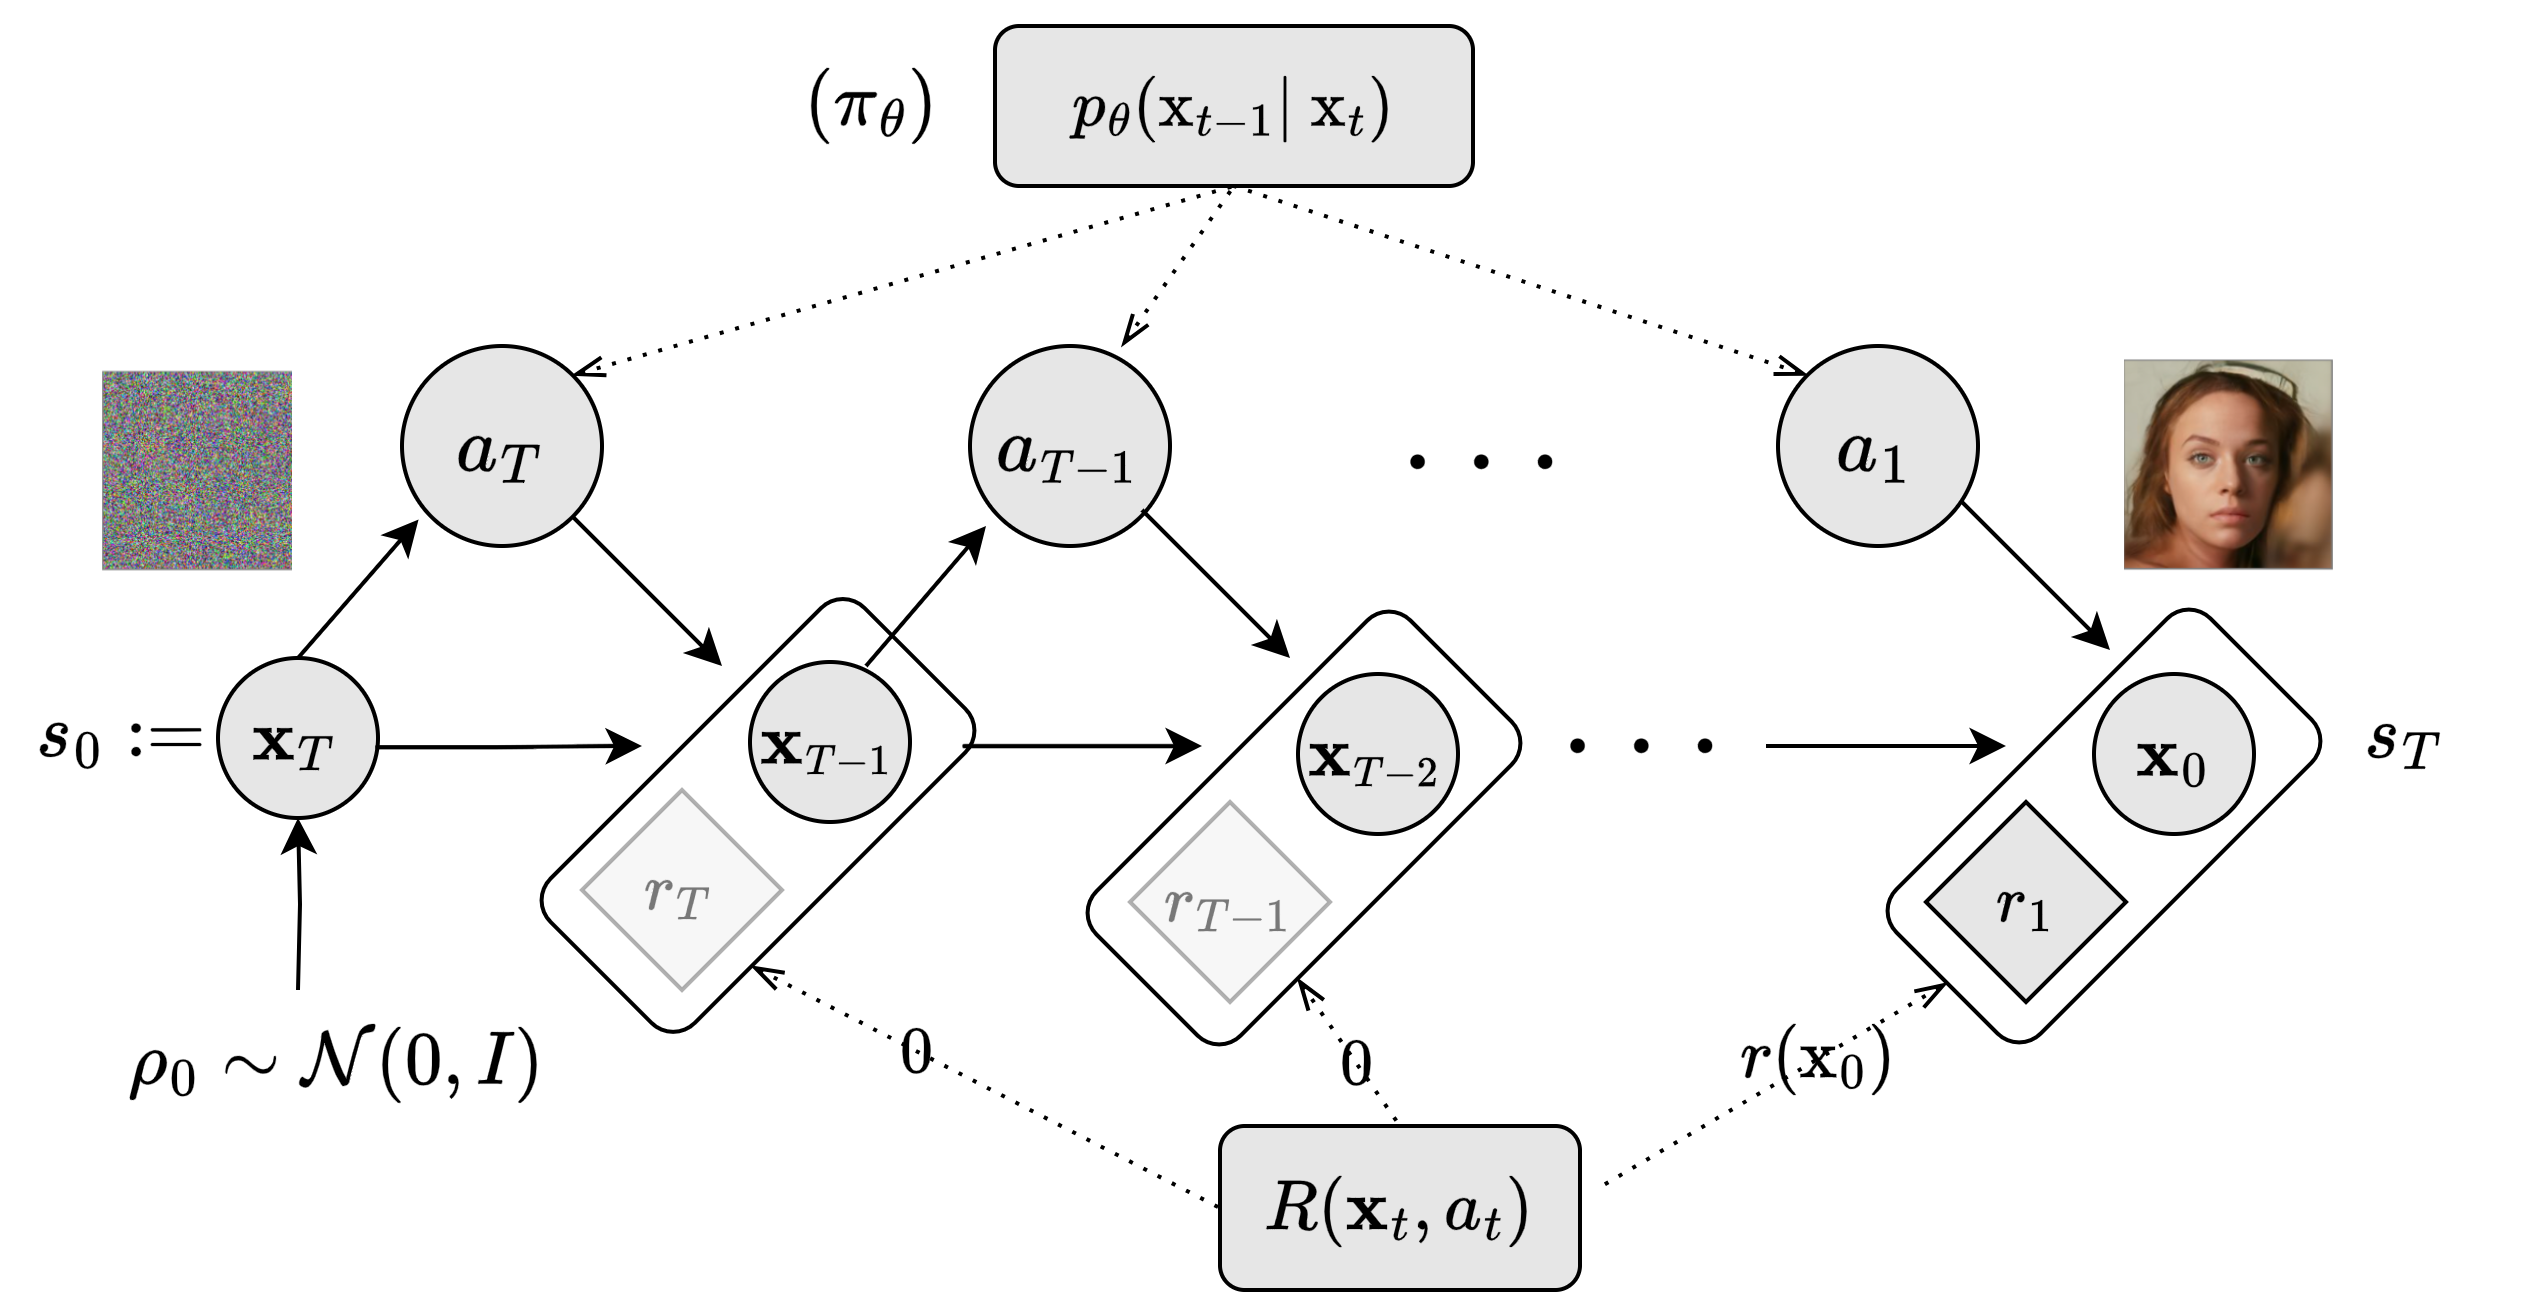
\includegraphics[scale=0.85]{img/results/diffusion-model-MDP.png}
  \vspace{-4pt}  % reduce space between caption and figure
    \captionsetup{width=\textwidth} % set the width of the caption
    \caption{\textbf{Diffusion model as a sequential decision-making process.} The policy
  $\pi_{\theta}:=p_{\theta}(\mathrm{x}_{t-1} | \mathrm{x}_{t})$ start taking denoising decisions from pure noise until the final sample $\mathrm{x}_0$, through the entire backward process $\tau=\mathrm{x}_{T:0}$. \textbf{TODO:} mejorar este caption...}
  \label{fig:diffusion-model-mdp}
\end{figure}

% agregar función de reward...
We consider the denoising diffusion policy optimization (DDPO) 
\cite{black2023training} formulation as starting point. The initial state
$\mathrm{s}_{0}$ is sampling from an isotropic Gaussian distribution
 $\rho_{0}\sim\mathcal{N}(0, I)$, corresponding to the noise
 $\mathrm{x}_{T}$ at the beginning of the diffusion backward process (Figure~\ref{fig:diffusion-model-mdp}), when the
sampling process start. The denoising neural network $p_{\theta}$ using to
estimate $\mathrm{x}_{t-1}$ at each timestep $t$ directly, or indirectly by
estimate the noise $\hat{\epsilon}_{t}$, is treat as the policy
$\pi_{\theta}(a_{t}, s_{t})$, in which the agent via its denoising action moves 
from a noisy step to a less noisy one, i.e. $a_t: x_{t} \rightarrow x_{t-1}$.

In this framework, we can optimize the diffusion model parameters 
$\theta$ directly via policy gradient estimation to maximize any arbitrary
scalar-reward signal over the sample $\mathrm{x}_{0}$ producing by the diffusion
process, using the following objective:
\begin{equation}\label{difusion-rl-objective-1}
  \mathcal{J}_{\text{DDRL}}(\theta)
  = \mathbb{E}_{\mathrm{c}\sim p(\mathrm{c}),  \mathrm{x}_{0}\sim p_{\theta}(\mathrm{x}_{0}|\mathrm{c})}[ r(\mathrm{x}_{0}, \mathrm{c})]
\end{equation}
An important point of this formulation is that the reward $R(s_{t}, a_{t})$
only provide information from the final sample $\mathrm{x}_{0}$, giving zero
reward to every non-terminal state, or $\mathrm{x}_{t}$ where $t\neq0$ as it is
depicted in Figure~\ref{fig:diffusion-model-mdp}.

Given the objective of this agent, the DDPO works presents two objective 
variations, the traditional REINFORCE objective \cite{williams1992simple} called $\text{DDPO}_{\text{SF}}$, where SF stand by score function method to estimate gradients from samples using Monte Carlo \cite{mohamed2020monte}, and $\text{DDPO}_{\text{IS}}$ that used importance sampling to optimize a surrogate objective \cite{schulman2015trust} \cite{schulman2017proximal}.
% agregar objetivo DDPO_{SF}
\begin{equation}\label{eqn:ddpo-sf-objective}
  (\text{DDPO}_{\text{SF}})~~ \nabla_{\theta}\mathcal{J} = \mathbb{E}_{\mathrm{x}_{T:0}\sim p_{\theta}} \bigg[\sum_{t=0}^{T}\nabla_{\theta}\log p_{\theta}(\mathrm{x_{t-1}|\mathrm{x}_t}) r(\mathrm{x}_{0})\bigg]
\end{equation}
% agregar objetivo DDPO_{IS}
\begin{equation}\label{eqn:ddpo-is-objective}
  (\text{DDPO}_{\text{IS}})~~ \nabla_{\theta}\mathcal{J} = \mathbb{E}_{\mathrm{x}_{T:0}\sim p_{\theta_{\text{old}}}} \bigg[\sum_{t=0}^{T}\frac{p_{\theta}(\mathrm{x}_{t-1}|\mathrm{x}_{t})}{p_{\theta_{\text{old}}}(\mathrm{x}_{t-1}|\mathrm{x}_{t})}\nabla_{\theta}\log p_{\theta}(\mathrm{x_{t-1}|\mathrm{x}_t}) r(\mathrm{x}_{0})\bigg]
\end{equation}
It is straightforward to compute $\log p_{\theta}$ considering that
$p_{\theta}$ is a conditional gaussian distribution 
$\mathcal{N}(f_{\theta}(\mathrm{x}_{t}) | \mathrm{x}_{t-1}, \alpha)$, where
$f_{\theta}$ is a neural network such as U-net architecture parameterized by $\theta$.

\section{Extending RL in diffusion models}

Simplifying the problem and ignoring the context raise from conditional generative models such as text-to-image, instead we assume an unconditional model free of context. Following...
\begin{equation}\label{difusion-rl-objective-2}
  \mathcal{J}_{\text{DDRL}}(\theta)
  = \mathbb{E}_{\mathrm{x}_{0}\sim p_{\theta}(\mathrm{x}_{T:0})}[R(\mathrm{x}_{T:0})]
\end{equation}

Based on the summarization of policy gradients in \cite{schulman2015high} we can see the design decision to extend reinforcement learning, these are non excluyentes...
\begin{equation}\label{eqn:general-pg-estimation-form}
  \nabla_{\theta}\mathcal{J}(\theta) = \mathbb{E}\bigg[\sum_{t=0}^{\infty}\Psi_{t}\nabla_{\theta}\log\pi_{\theta}(a_{t}|s_{t}) \bigg]
\end{equation}
La idea es que cualquier mejora de propuesta, utilice o no conocimientos
desde el campo de modelos de difusión, caiga en alguna de las siguientes
formulaciones para la optimización de policy gradient methods presentada
en el paper \textit{High-Dimensional Continuous Control Using Generalized Advantage Estimation}, aka GAE.

\subsection{Total Reward of the Trajectory}

\begin{equation}\label{eqn:psi-total-reward}
  \sum_{t=0}^{\infty}\Psi_{t} = \sum_{t=0}^{\infty} r_{t}
\end{equation}


\subsection{Reward following Action}

Reward on to go...

\begin{equation}\label{eqn:psi-reward-following-action}
  \sum_{t=0}^{\infty}\Psi_{t} = \sum_{t=t'}^{\infty} r_{t'}
\end{equation}

\subsection{Reward following Action with Baseline}

\begin{equation}\label{eqn:psi-reward-following-action-baseline}
  \sum_{t=0}^{\infty}\Psi_{t} = \sum_{t=t'}^{\infty} r_{t'} - b(s_{t})
\end{equation}


\subsection{MaDI: a masker to turn off non-informative pixels}

XYZ

\section{Empirical Analysis of Reward Trajectory Dynamics: Insights from DDPM samples}

¿Porqué valdría la pena extender el reward? ¿los estados intermedios 
aportan información?

% Reward signal during samples trajectories 
\begin{figure}[ht]
  \centering
  \begin{minipage}{0.5\textwidth}
      \centering
      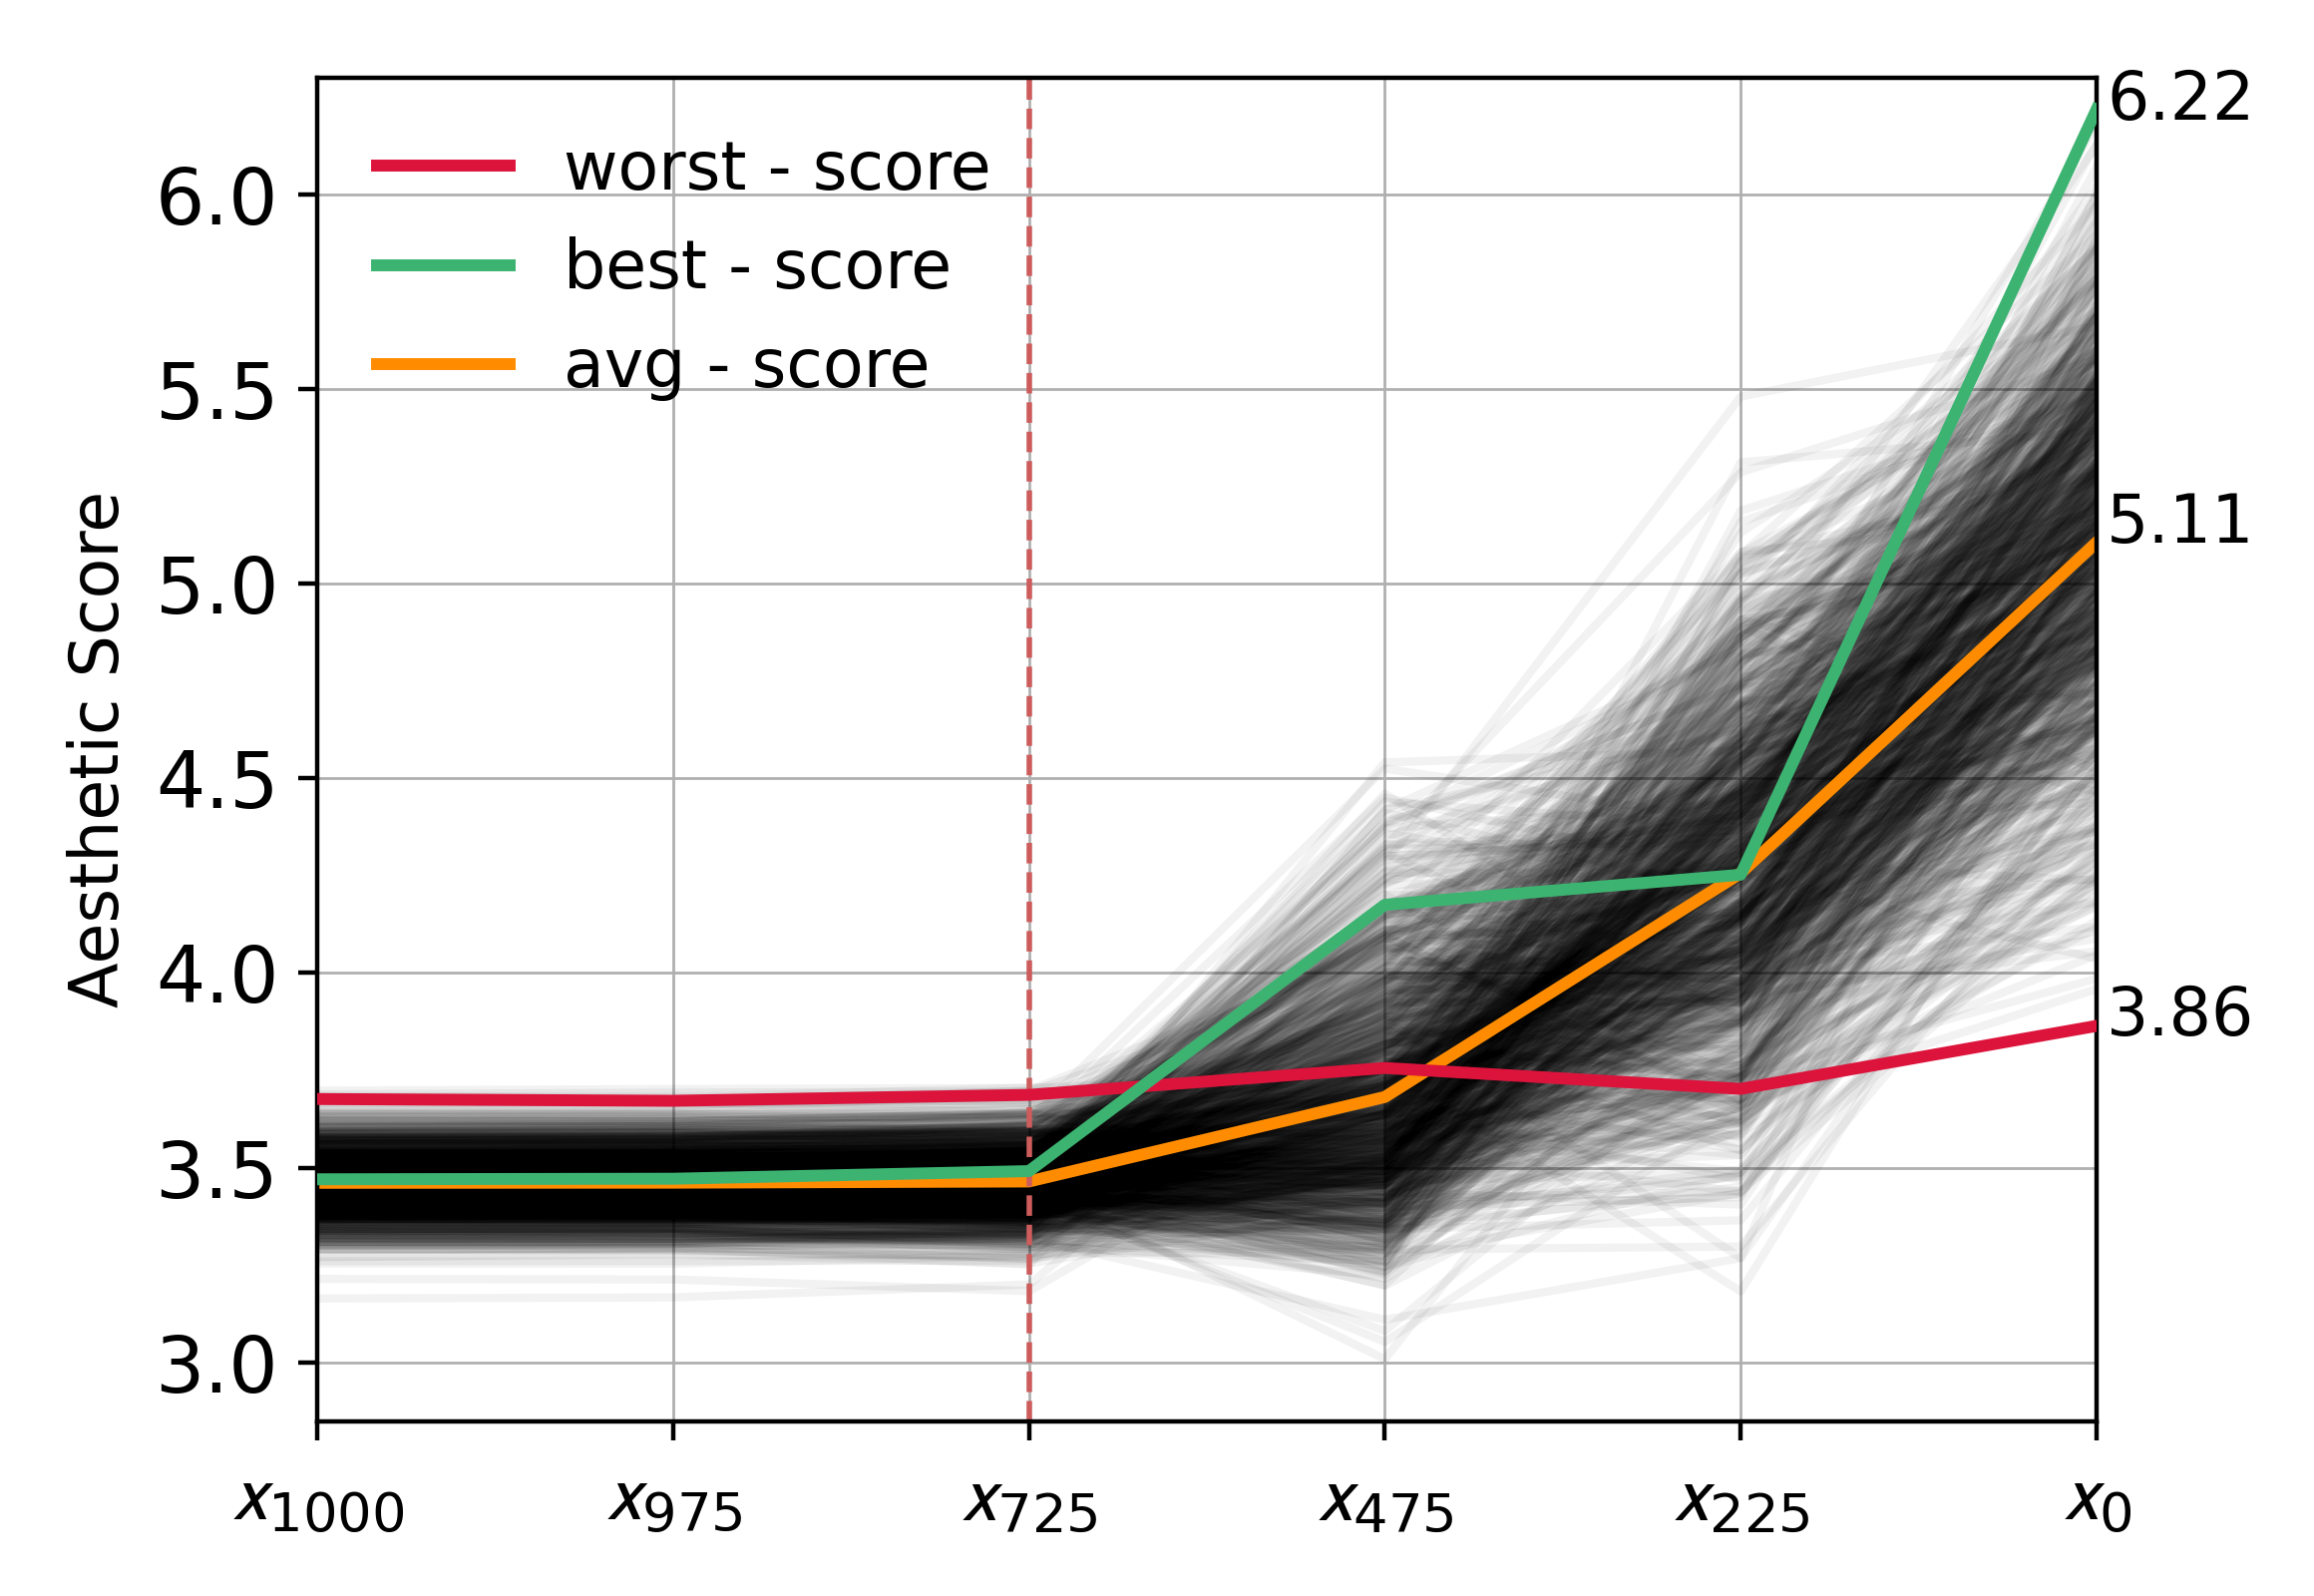
\includegraphics[width=1\textwidth]{img/results/1k-trajectories-aestheic-score-single.png} % first figure itself
  \end{minipage}\hfill
  \begin{minipage}{0.5\textwidth}
      \centering
      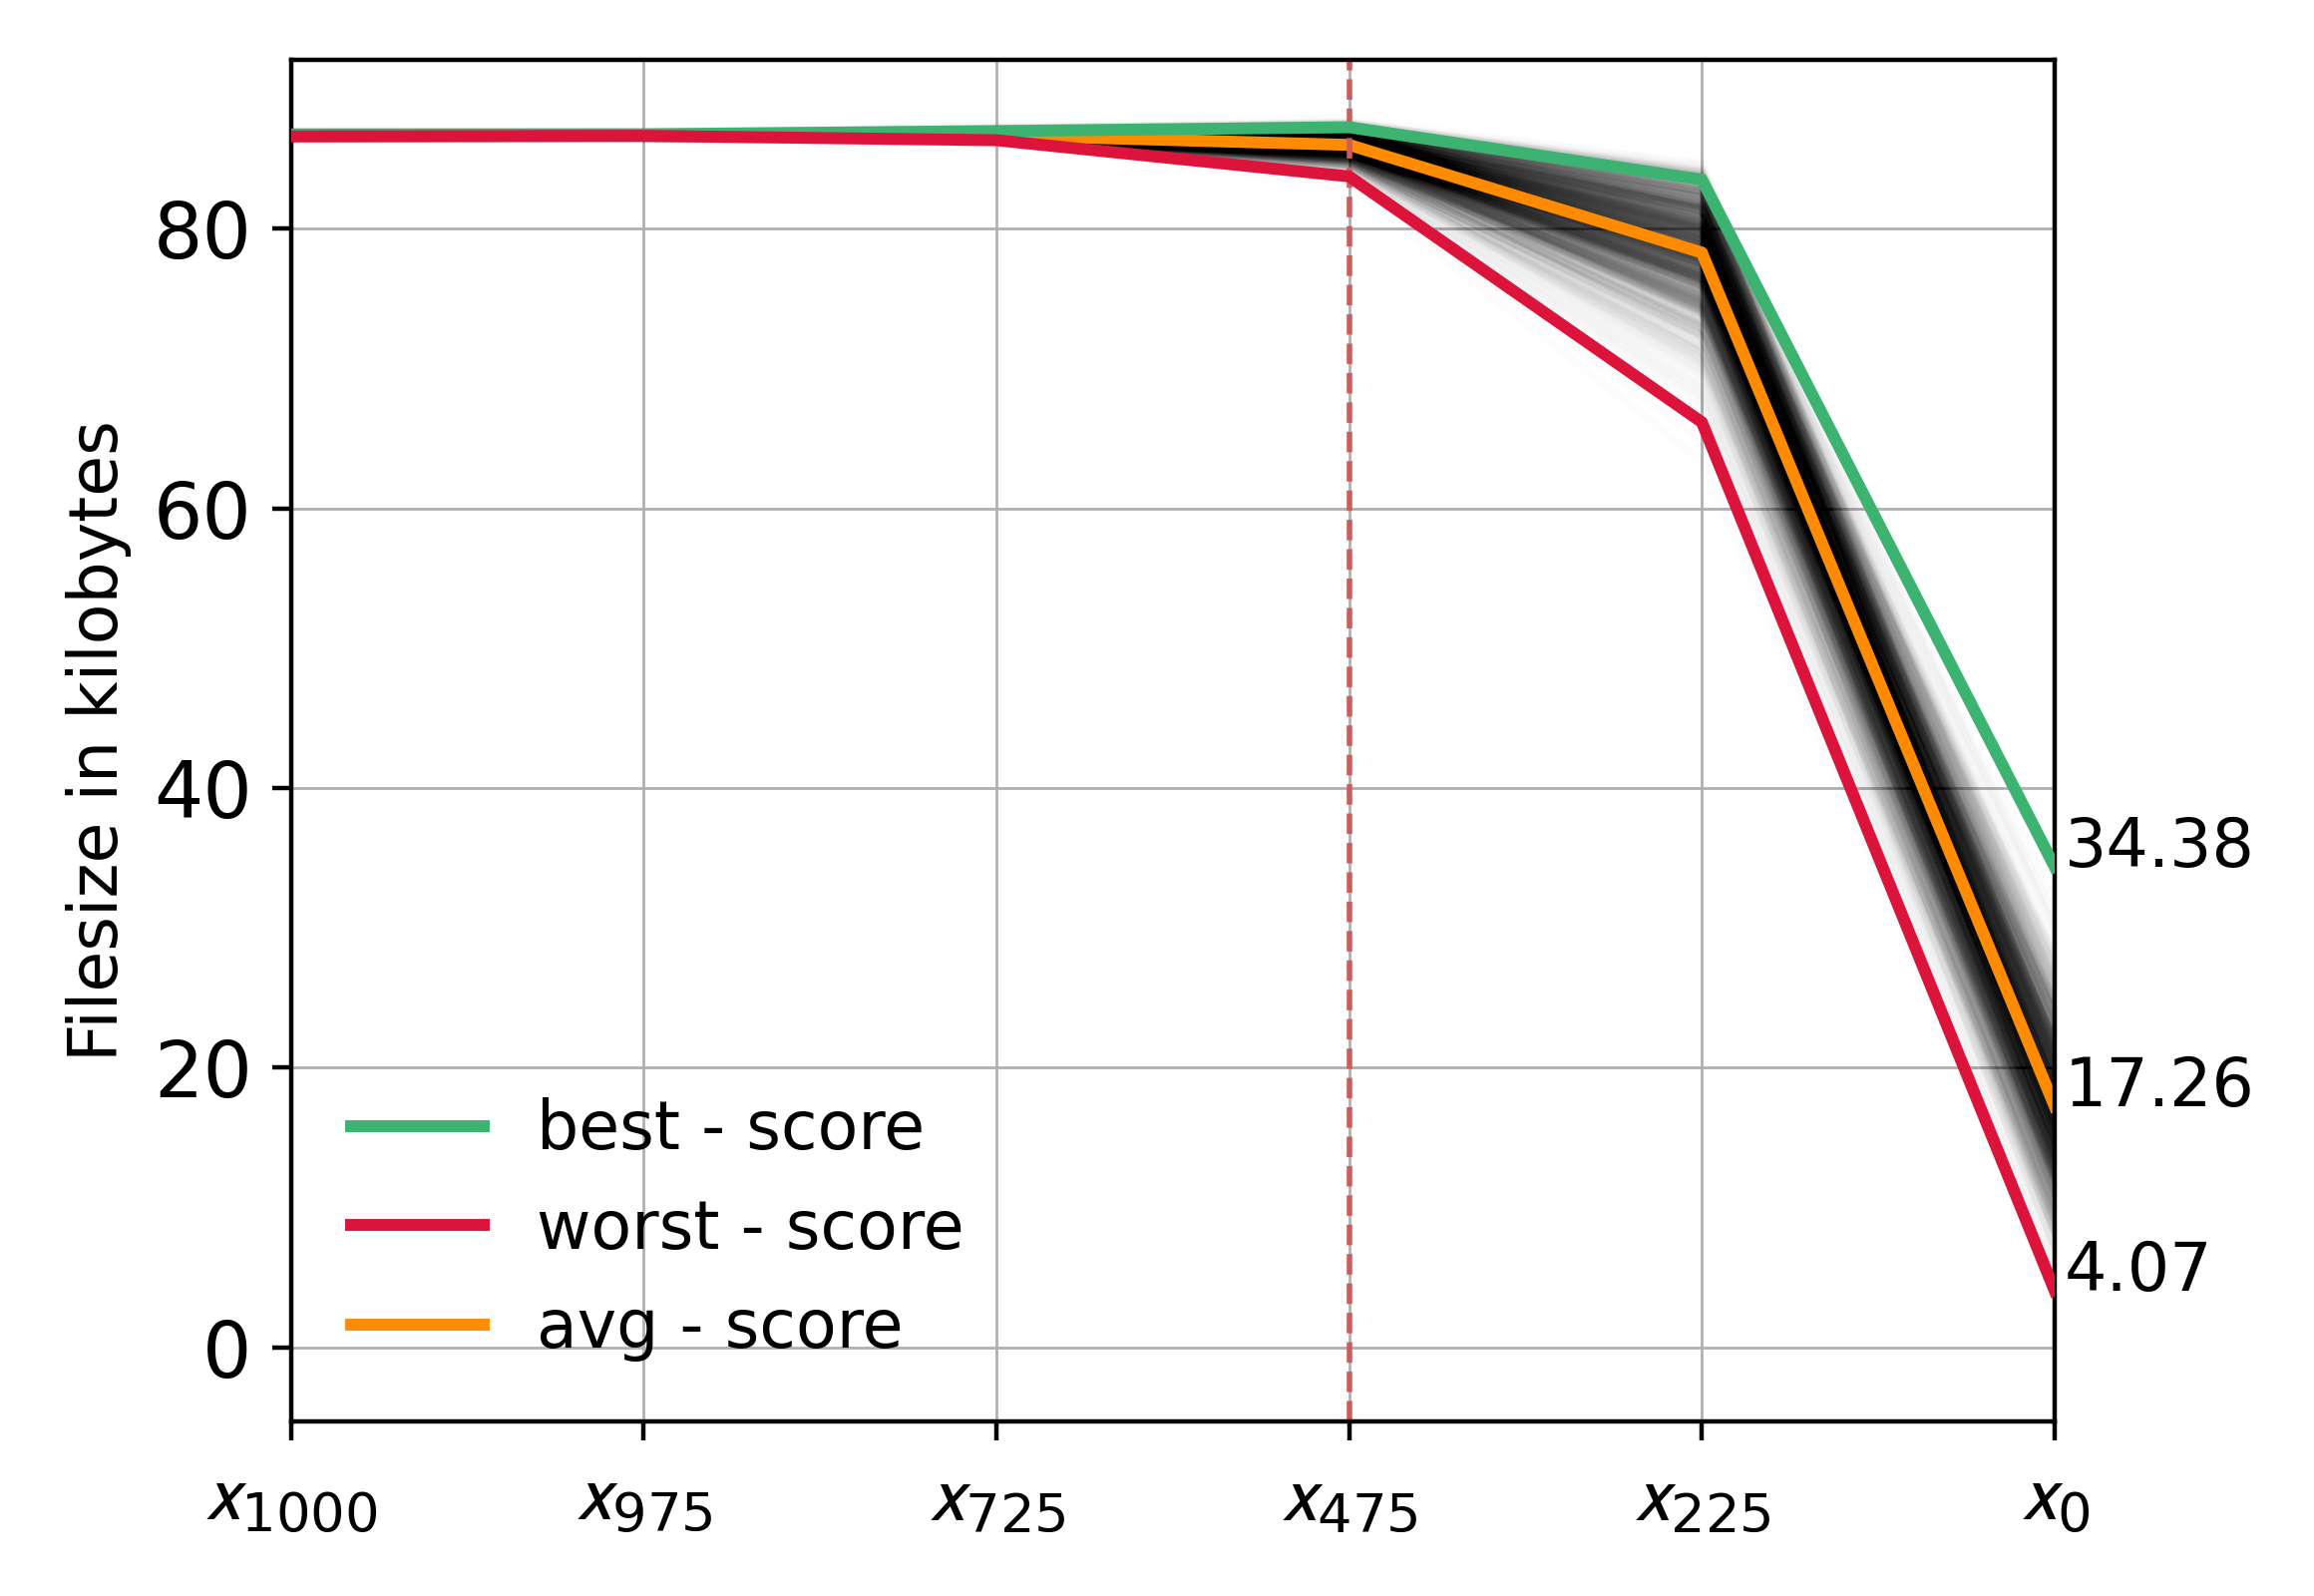
\includegraphics[width=1\textwidth]{img/results/1k-trajectories-jpeg-size-single.png} % second figure itself
  \end{minipage}
  \vspace{-8pt}  % reduce space between caption and figure
    \captionsetup{width=\textwidth} % set the width of the caption
    \caption{\textbf{Visualizing reward signal during sample trajectories.} \textbf{Left:} Evolution of the aesthetic quality as reward signal over the six states $\mathrm{x}_{\tilde{t}}$, summarizing each of the $1000$ trajectories. \textbf{Right:} Image size after JPEG compression, providing another form of reward signal for the same set of trajectories.}
  \label{fig:samples-trajectory-rewards} % Add a proper reference for the label
\end{figure}


We utilize the \texttt{google/ddpm-celebahq-256} diffusion model \cite{ho2020denoising} to compile a dataset of trajectory samples, denoted as $\mathcal{S}_o$. This dataset comprises summaries of six intermediate states extracted from each trajectory. We specifically consider steps $t$ within the range of $0$ to $1000$, where the model was trained. To move from the final state of the diffusion chain, which is Gaussian noise, to the initial state, we leverage the reverse process of the diffusion chain.

Our methodology involves summarizing the sample trajectories by selecting intermediate steps at specific timestamps. We opted for a trajectory length of 40 steps, and interpolated within the original diffusion chain using the \texttt{DDIMScheduler} \cite{song2020denoising}. While obtaining the reward for the entire trajectory involves evaluating it over 40 times the original steps, we collect the rewards for every tenth step for memory and computational efficiency. Alternative approaches for selecting significant intermediate steps could be explored in future work.

Each state in the dataset is associated with a reward signal, which can be obtained using parameterized models such as the LAION aesthetic predictor or the ViT age classifier, or through functions like JPG compression size estimation.

\begin{enumerate}
\item The $\tilde{t}$ specified a subset of the step $t$ within the diffusion chain $t=0, \dots, T=1000$, in which the model \texttt{google/ddpm-celebahq-256} was trained.
\item Equivalence between $\tilde{t}$ and $t$ is given in the following tuples:
$(\tilde{t}=0, t=1000), (\tilde{t}=1, t=975), (\tilde{t}=2, t=725), (\tilde{t}=3, t=475), (\tilde{t}=4, t=225), (\tilde{t}=5, t=0)$.
\item The intermediate steps $\mathrm{x}_{t}, ~t\notin [0,1000]$, were collected every ten steps from the 40-step trajectory length. The reason was for memory and computation. Obtaining the reward for the complete trajectory requires moving from $6N$ to $40N$ reward evaluations.
\item Therefore, the dataset of samples $\mathcal{S}_{o} =  \big\{\mathrm{x}_{\tilde{t}}^{(i)}, \mathrm{r}_{\tilde{t}}^{(i)} \big\}_{\tilde{t}=0:5}~$, describe each $i$ trajectory from a total of $N$.
\end{enumerate}
%\item Every state has a $r\in \mathbb{R}$, corresponding to a reward. This signal can be obtained by a parameterized model such as \href{https://laion.ai/blog/laion-aesthetics/}{LAION aesthetic predictor} or \href{https://huggingface.co/nateraw/vit-age-classifier}{ViT age classifier}, or from functions such as obtaining the size of an image after JPG compression.

In Figure~\ref{fig:samples-trajectory-rewards} we can inspect...\\

Analyze the reward over predicted samples given an intermediate
state $\mathrm{x}_{t}$. \textit{Are intermediate samples with higher/lower reward as correlated with their predicted reward at the final sample?} We
will use the sample prediction $\tilde{\mathrm{x}}$ obtained by DDIM
\begin{equation}\label{ddim-predicted-sample}
  \tilde{\mathrm{x}}_{0}=\text{pred}(\mathrm{x}_{t})=\frac{\mathrm{x}_{t}-\sqrt{1-\alpha_{t}}\epsilon_{\theta}^{(t)}(\mathrm{x}_{t})}{\sqrt{\alpha_{t}}}
\end{equation}

¿Tiene lógica ver el \textit{reward} acumulado de una trayectoria completa?
¿No es un mal estimado el \textit{reward} un estado intermedio dado el ruido?

% No aporta muchoo el ruido
\begin{figure}[ht]
  \centering
  \includegraphics[scale=0.80]{img/results/samples-trajectories.png}
  \vspace{-18pt}  % reduce space between caption and figure
    \captionsetup{width=\textwidth} % set the width of the caption
    \caption{\textbf{DDPM samples trajectories.} Each row, from \textbf{top-to-bottom}, represents the best ($6.22$)
  and worst ($3.86$) aesthetic scores, and the highest ($34.38$) and lowest 
  ($4.07$) filesizes in kilobytes after JPEG compression for samples
  $\mathrm{x}_{0}$ in $\mathcal{S}_{o}$. Each column, from \textbf{left-to-right}, summarizes the
  states for each sample's trajectory. The rows correspond to the trajectories
  highlighted in the green and red lines of Figure~\ref{fig:samples-trajectory-rewards}}.
    \label{fig:sample-trajectories}
\end{figure}

\section{Model}

XYZ

\section{Experiments}

En primer lugar queremos reproducir la implementación propuesta en \textit{Training Diffusion Models with Reinforcement Learning} \cite{black2023training} en un \textit{setting} más simplificado para facilitar
la experimentación, pero que aún capture la complejidad de los text-to-image models para experimentar con \textit{reward functions}. Utilizaremos como
modelo preentrenado \texttt{google/ddpm-celebahq-256} descrito
en \cite{ho2020denoising}, el cual es un modelo no condicionado que
genera imágenes de dimensiones 256x256 de rostros humanos en RGB. Este modelo es previo a los modelos latentes de difusión, por lo que el proceso de \textit{denoising} ocurre en el espacio de los pixeles.


\subsection{LAION Aesthetic Score}

 XYZ

 \subsection{JPEG Compressibility \& Incompressibility}

 Using as a reward the size of the image after JPEG compression, we can 
 define two tasks: compressibility and incompressibility. For compressibility,
 we want to maximize the negative size of the image after compression. This
is equivalent to minimizing the size of the image after compression. 
The other side of the coin is to maximize the size of the image after compression, aka incompressibility.
  
 \subsection{Over 50 years old}

 XYZ

\begin{table}
\centering
\begin{tabular}{lccc}
\toprule
\textbf{Downstream Task} & \textbf{DDPM} & \textbf{DDPO} & \textbf{DDPOI}\\
\midrule
LAION Aesthetic Score ($[1,10]$) & 5.11 $~\pm$ 0.02 & \textbf{5.58} $~\pm$ 0.03 & - \\
JPEG compressibility (kb) & 17.26 $~\pm$  0.29 & \textbf{6.01} $~\pm$ 0.25  & -\\
JPEG incompressibility (kb) & 17.26 $~\pm$ 0.29 & \textbf{21.6} $~\pm$ 0.23 & - \\
Over 50 years old $P(x>\text{50})$ & 0.12 & - & - \\
\bottomrule
\end{tabular}
\captionsetup{width=\textwidth} % set the width of the caption
\caption{Mean and standard error of the mean (SEM) for rewards associated with each downstream task (rows) and each checkpoint trained based on the methods studied (columns). To ensure a fair comparison, all checkpoints were generated samples using the same initial noise. The \textbf{DDPM} column provides estimates of the initial capacities of the google/ddpm-celebahq-256 model, derived from the images in the dataset $\mathcal{D}_{o}$. The \textbf{DDPO} column corresponds to the checkpoint trained using DDPO with importance sampling, as referenced in \cite{black2023training}. The \textbf{DDPOI} column represents our proposed method. \textbf{TODO:} simplificar este caption mega verboso.}
\end{table}




% Mean and Reward Histograms for JPEG compressibility and incompressibility
\begin{figure}[ht]
  \centering
  \begin{minipage}{0.5\textwidth}
      \centering
      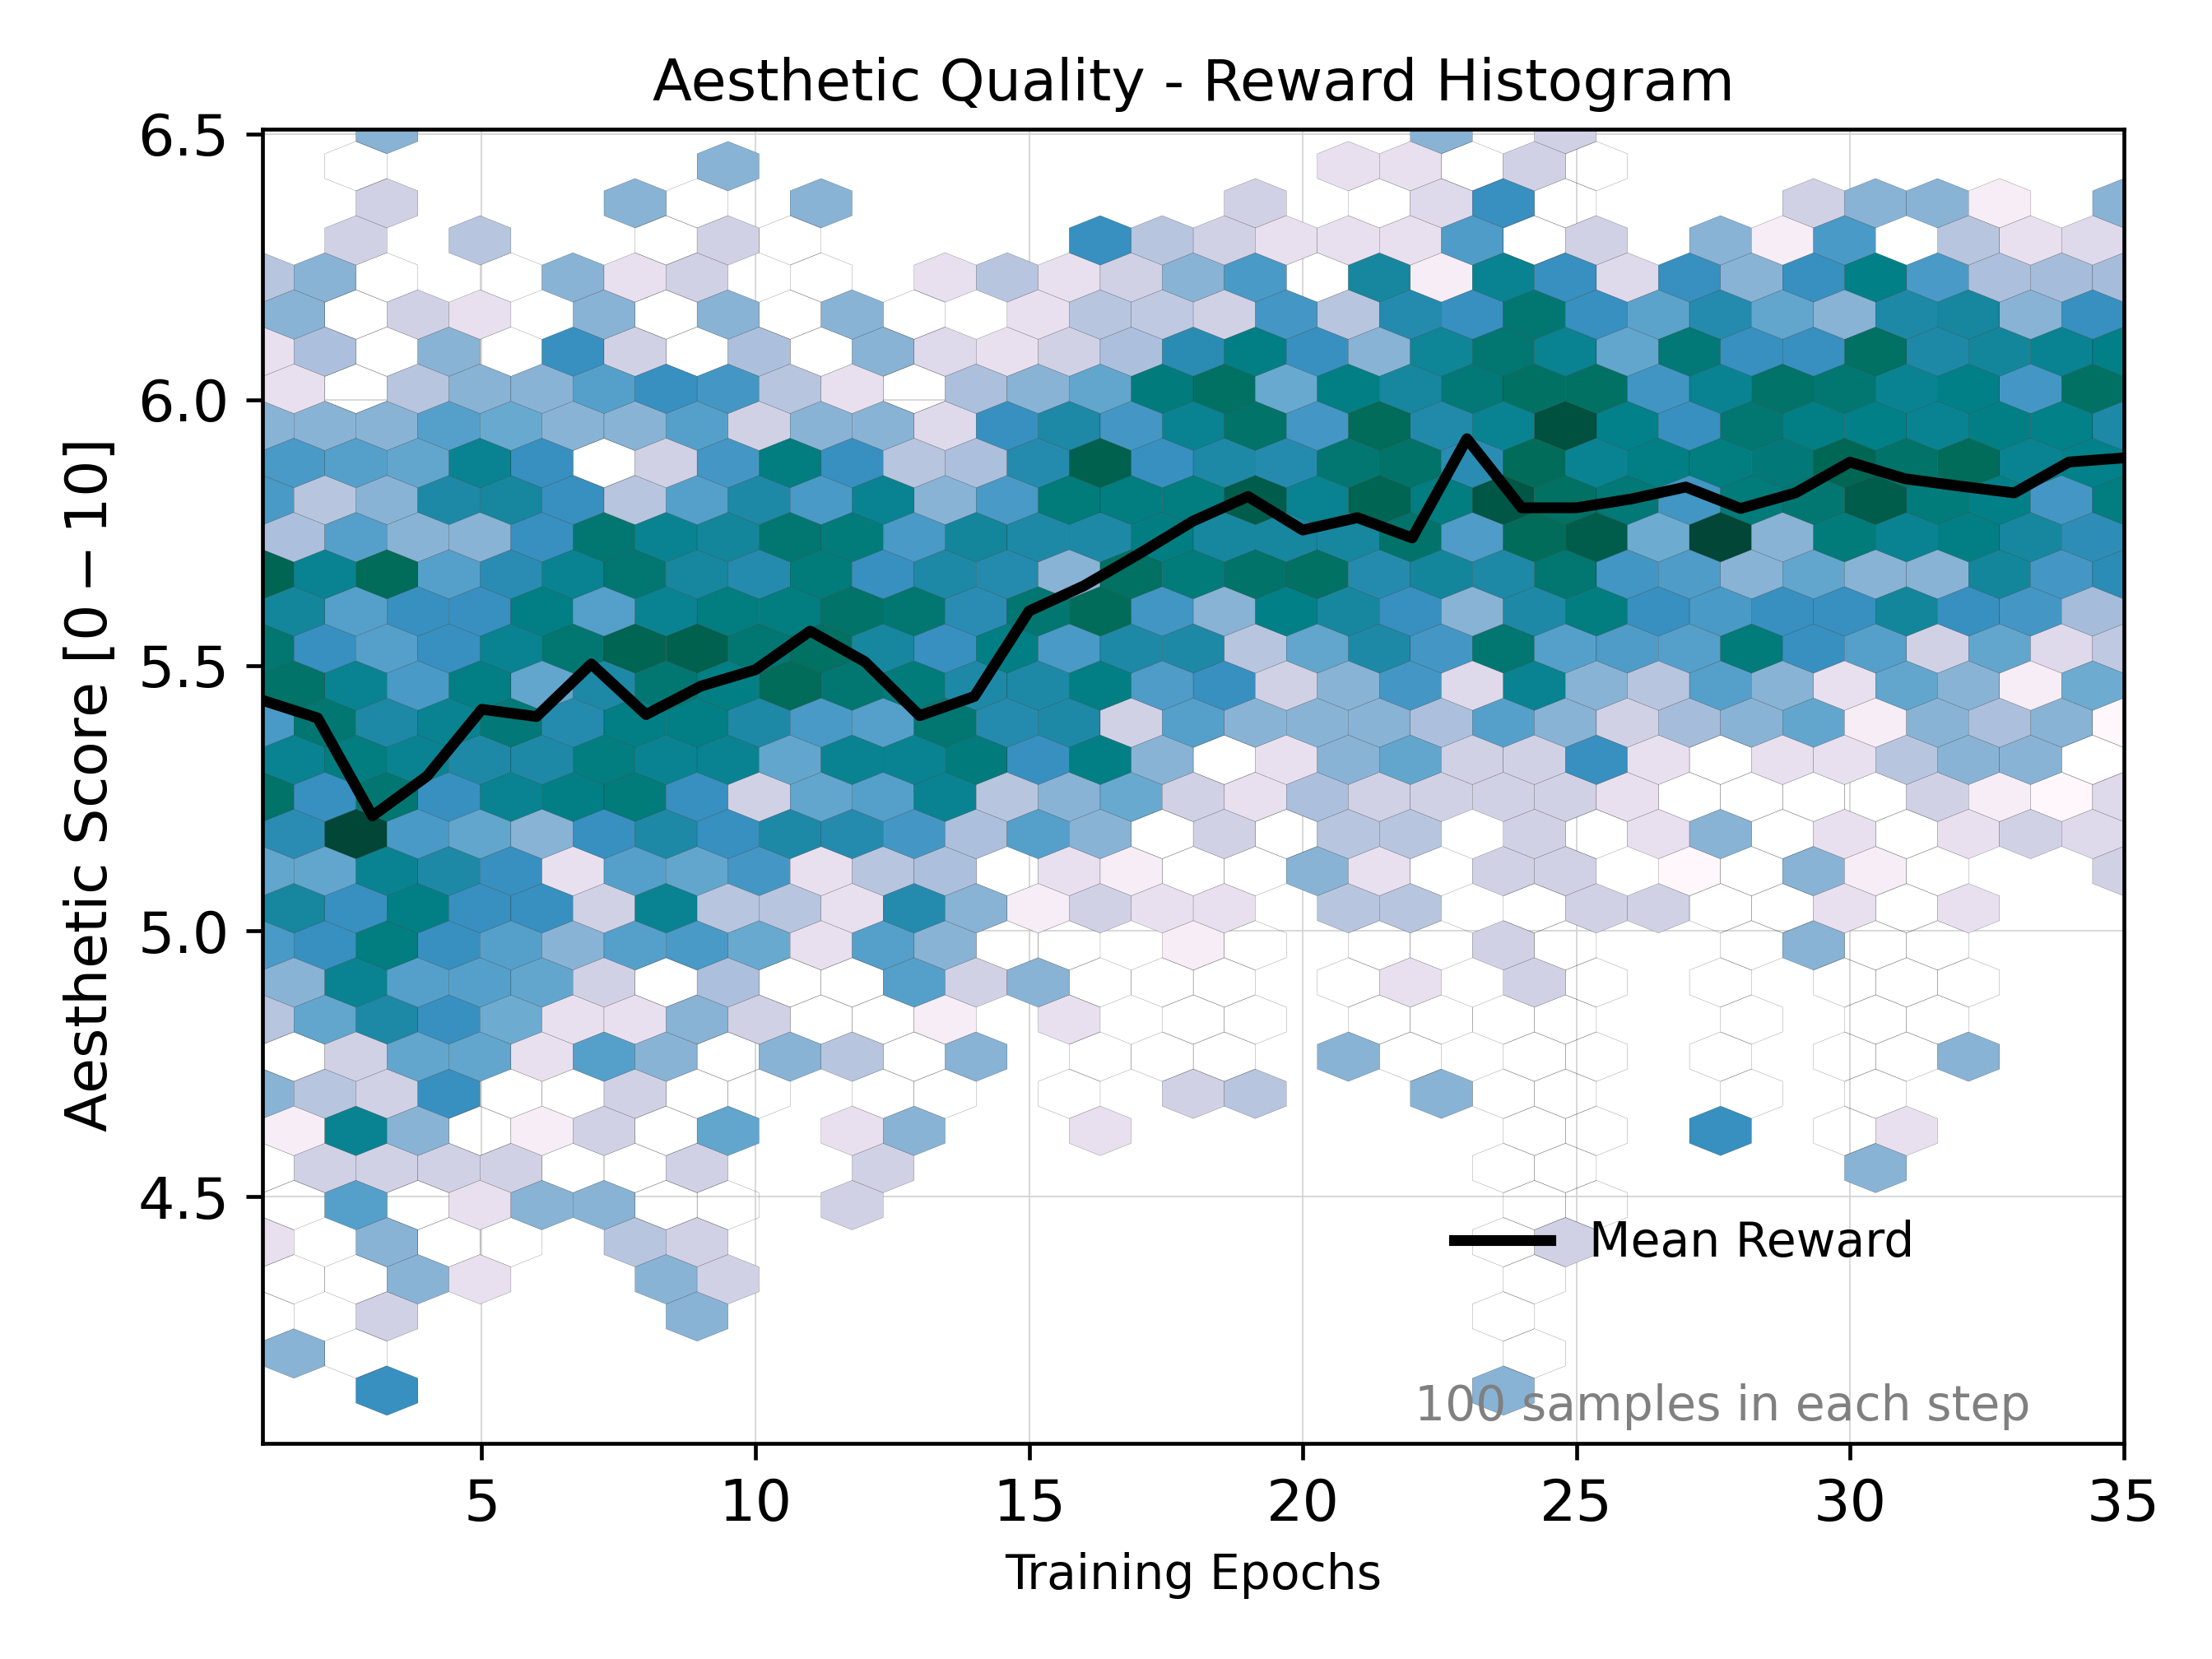
\includegraphics[width=1\textwidth]{img/results/reward_hist-laion-aesthetic.png} % first figure itself
      %\label{fig:sample_figure_1}
  \end{minipage}\hfill
  \begin{minipage}{0.5\textwidth}
      \centering
      % 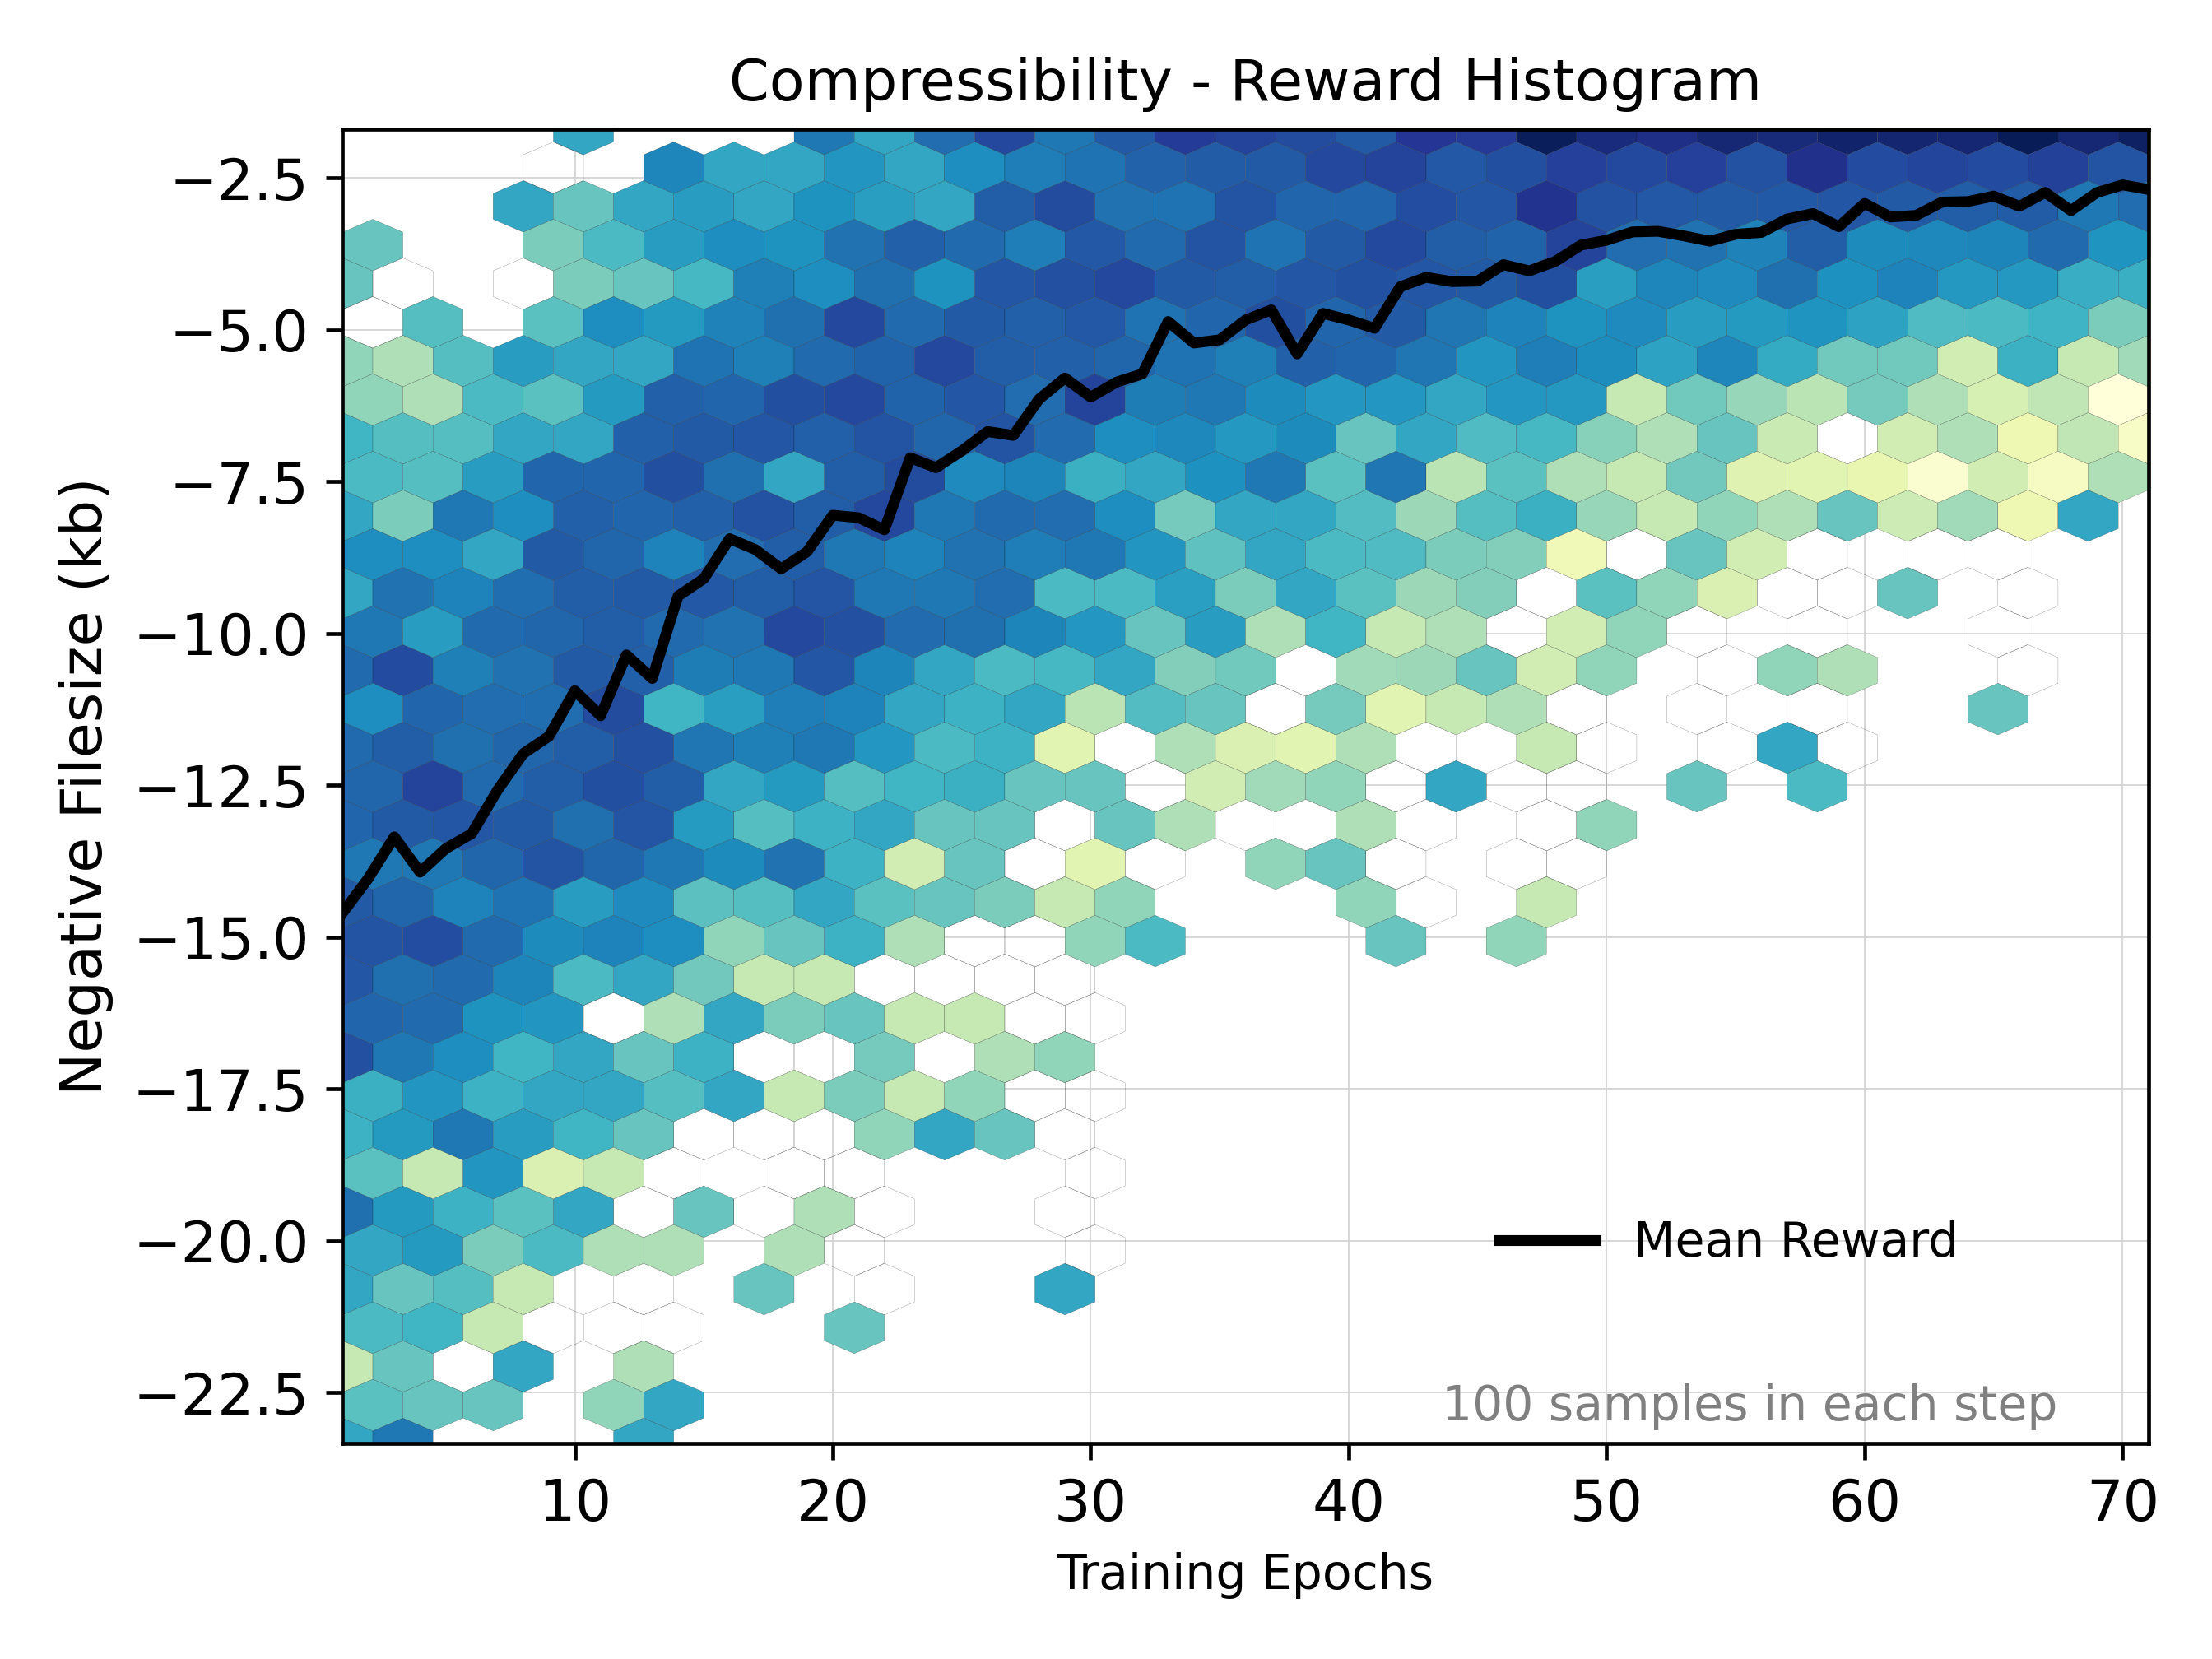
\includegraphics[width=1\textwidth]{img/results/reward_hist-jpeg-compressibility.png} % second figure itself
      %\label{fig:sample_figure_2}
  \end{minipage}\vspace{-0.1cm} % space between row 1 and row 2 of figures
  \begin{minipage}{0.5\textwidth}
      \centering
      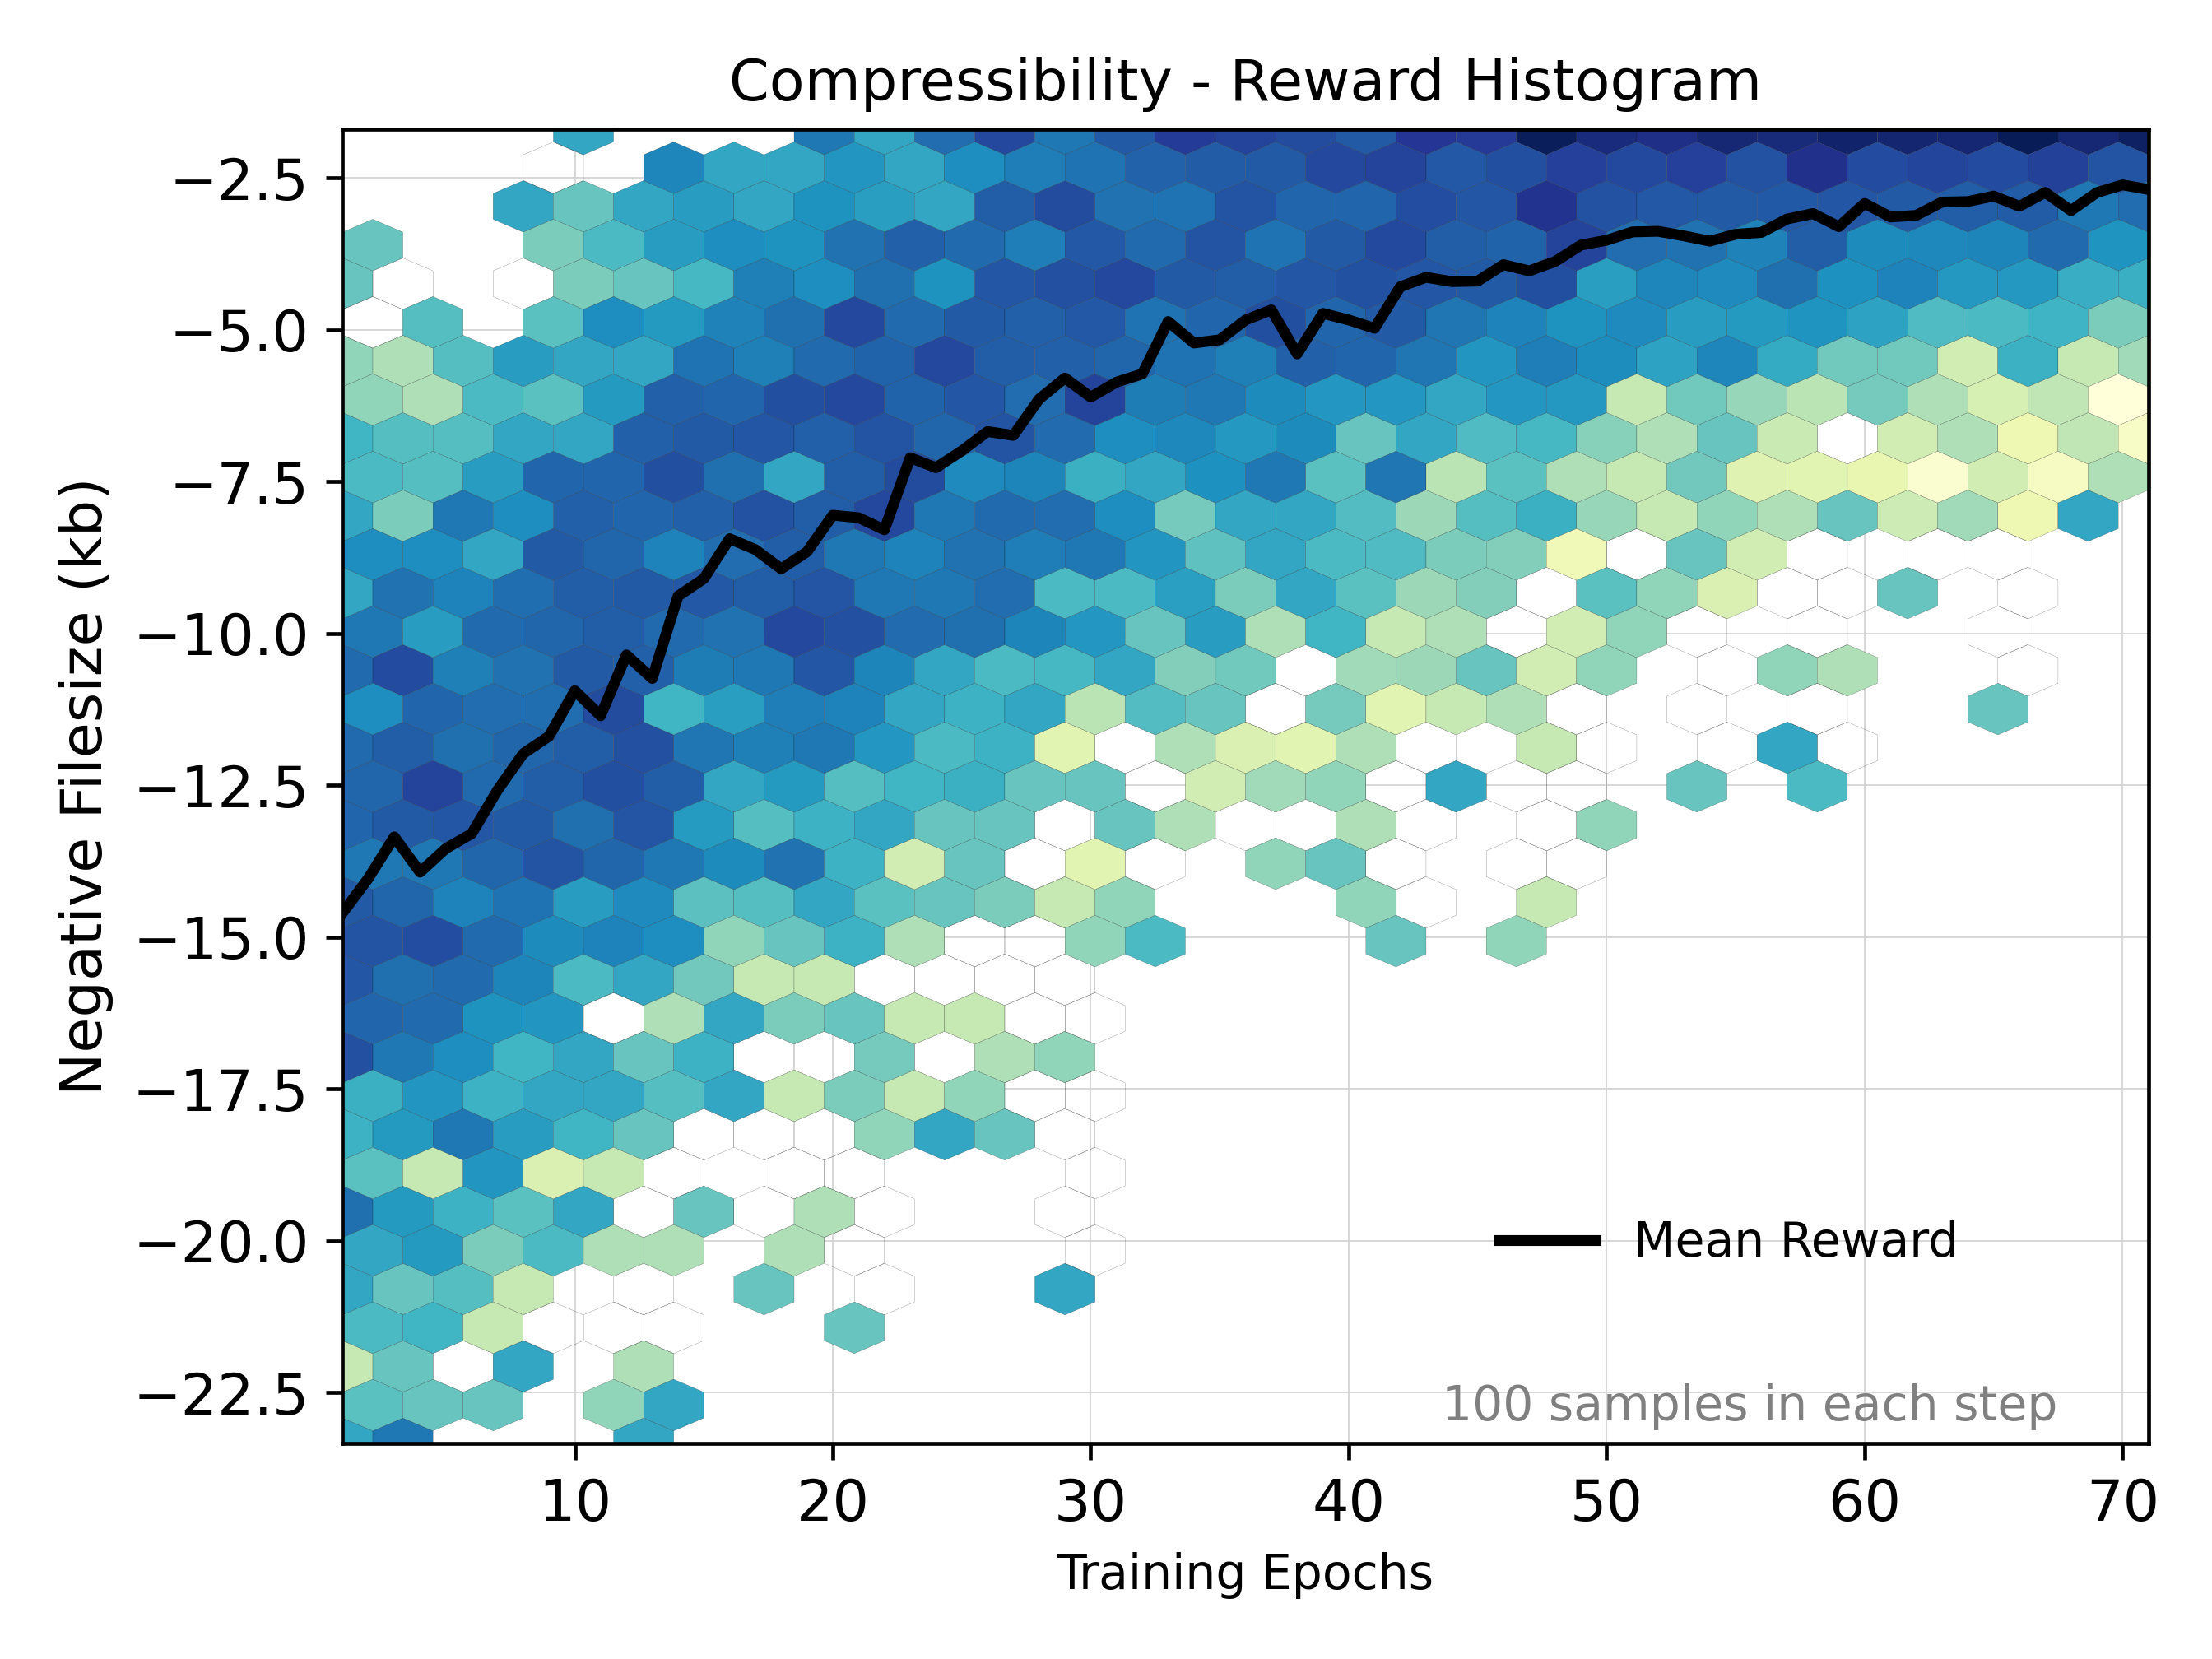
\includegraphics[width=1\textwidth]{img/results/reward_hist-jpeg-compressibility.png} % third figure itself
      %\label{fig:sample_figure_3}
  \end{minipage}\hfill
  \begin{minipage}{0.5\textwidth}
      \centering
      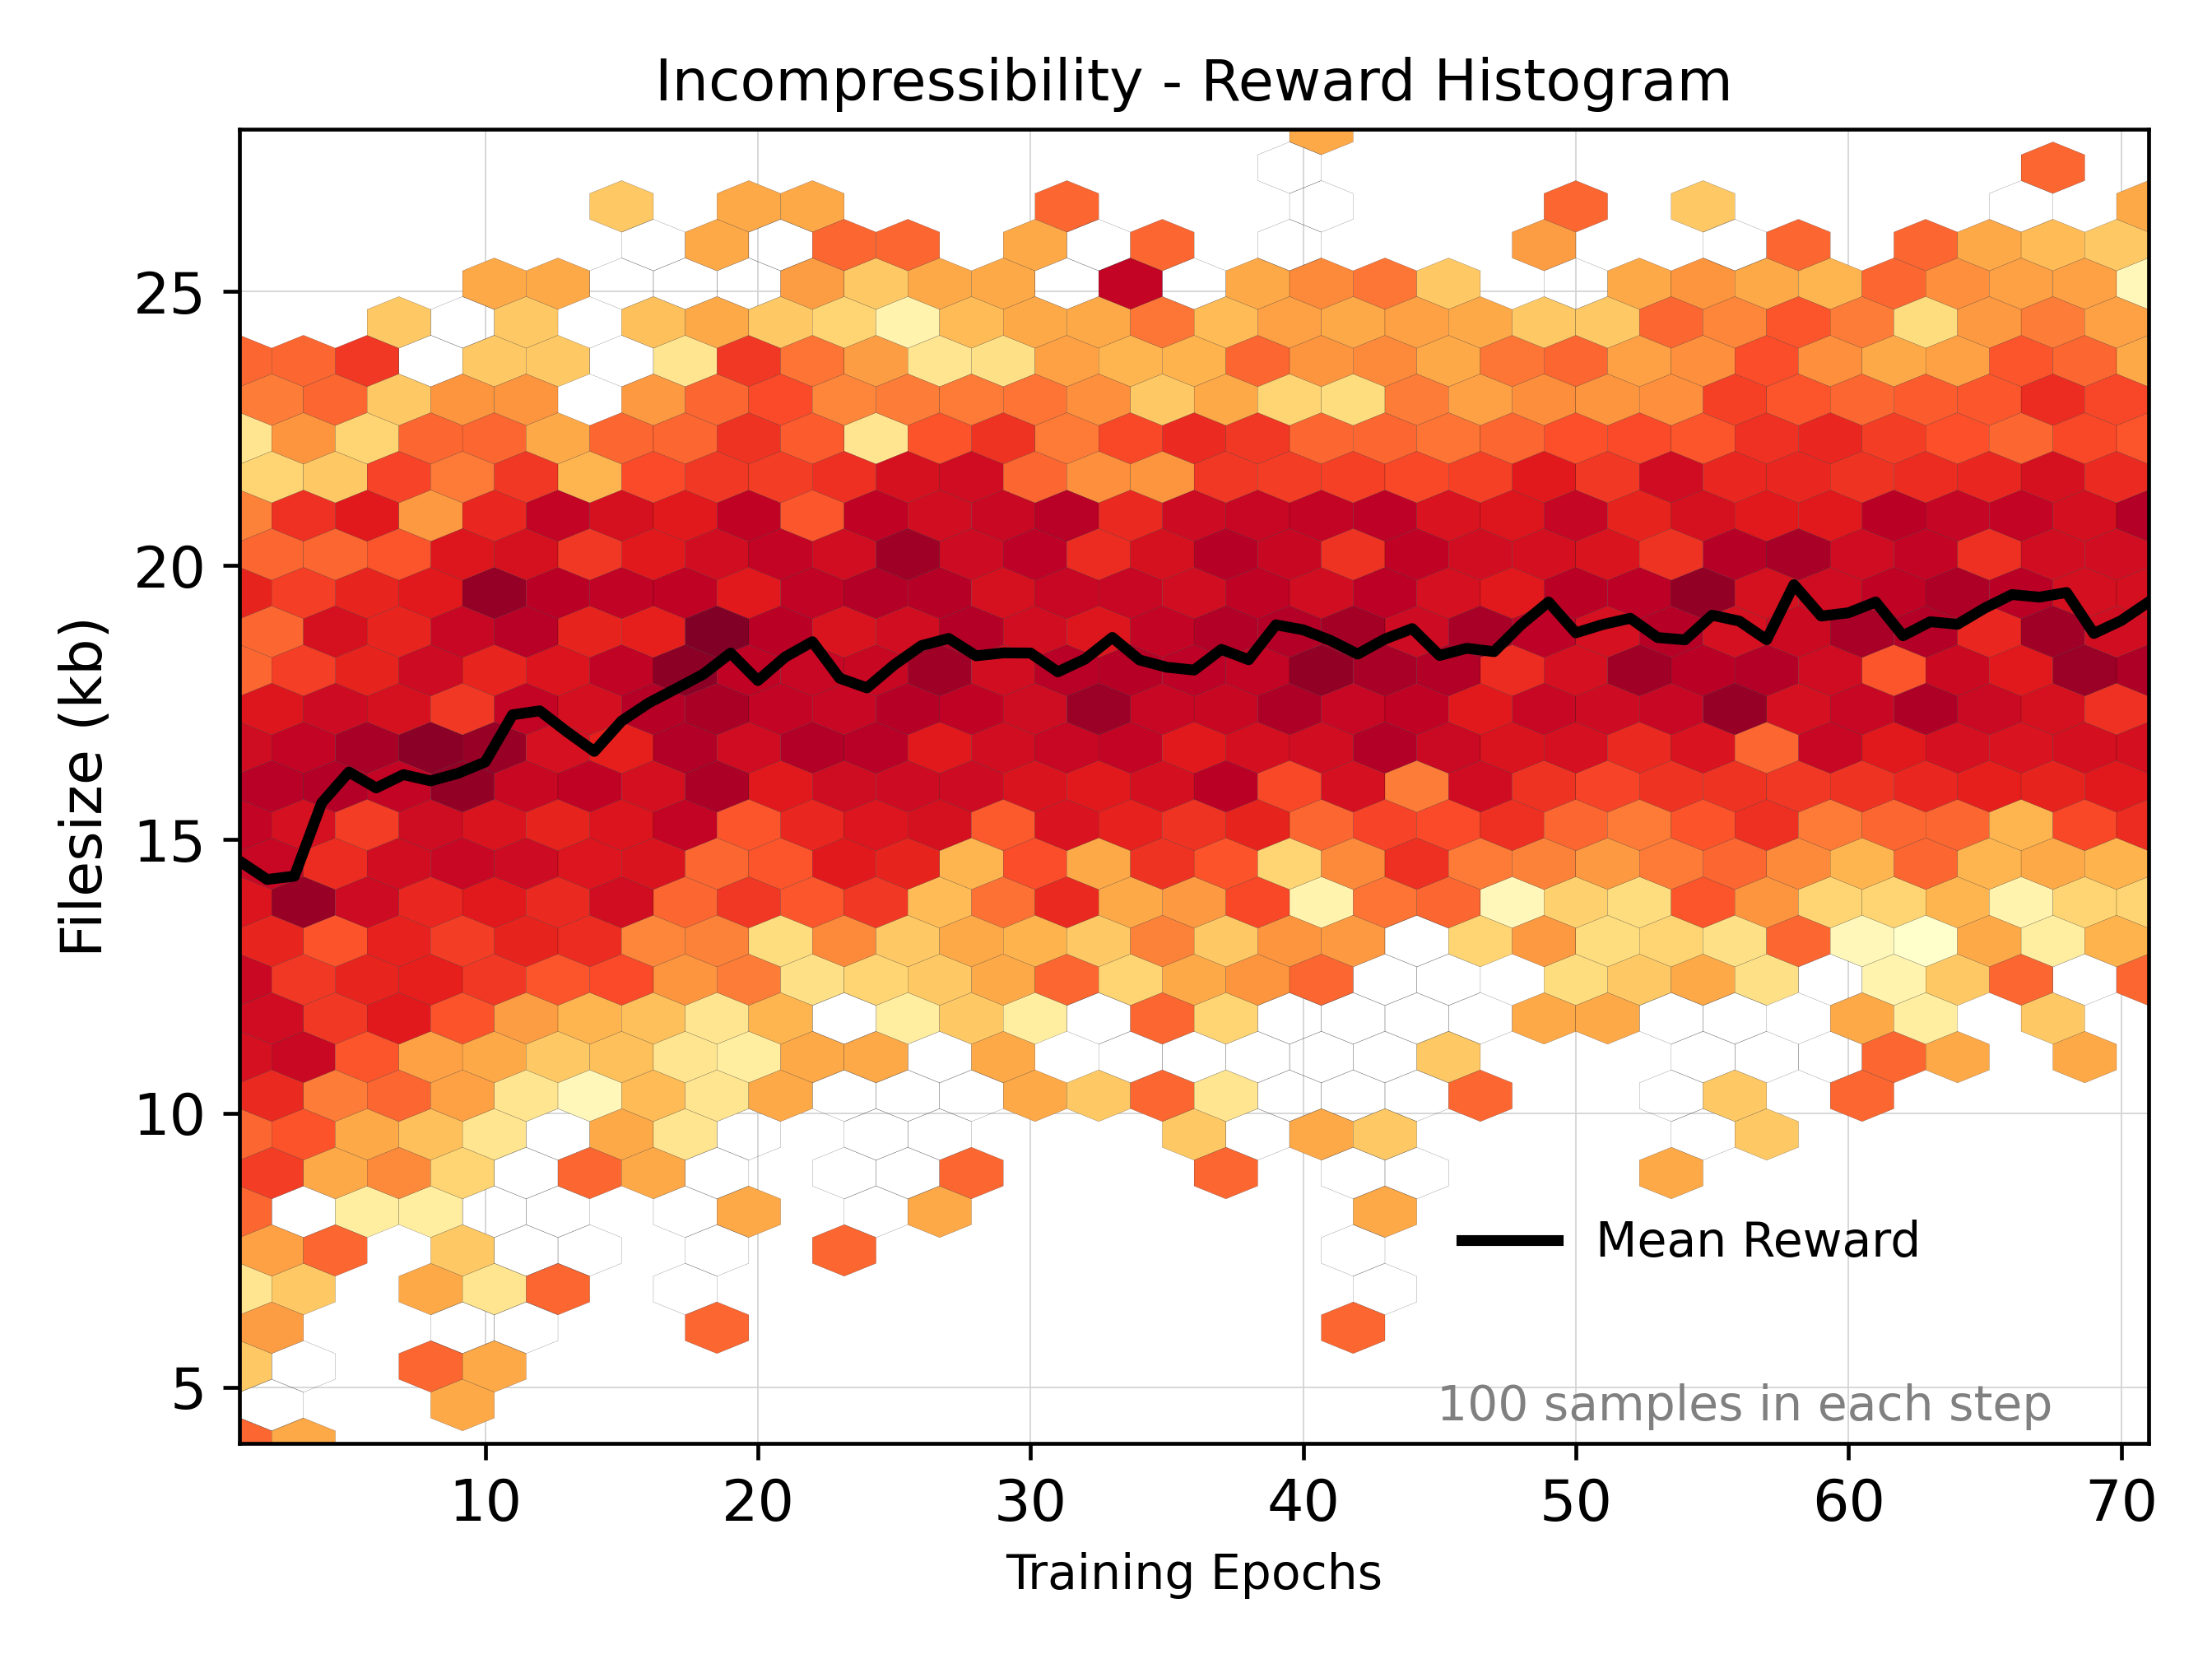
\includegraphics[width=1\textwidth]{img/results/reward_hist-jpeg-incompressibility.png} % forth figure itself
      %\label{fig:sample_figure_4}
  \end{minipage}
  \vspace{-8pt}  % reduce space between caption and figure
    \captionsetup{width=\textwidth} % set the width of the caption
    \caption{\textbf{Learning curves from DDPO.} Evolution of the mean reward (black line) and histogram during the training steps for each \textit{downstream task}. The reward estimates were computed in each step using $100$ samples from the model.}
  \label{fig:reward_hist} % Add a proper reference for the label
\end{figure}

Maximizar LAION aesthetic score es un task mucho más complejo que JPEG Compressibility y JPEG Incompressibility (Por ver).

JPEG Incompressibility resulta más difícil de maximizar JPEG Compressibility
(Figure~\ref{fig:reward_hist}). Lo que tiene sentido según la naturaleza del
task y las capacidades del modelo. Hasta cierto punto, añadir mayor información 
requiere de mayores capacidades generativas para agregar semantica visual y 
otros features dentro de la imagen que no se pierdan durante el proceso de
compresión. Sin embargo, reducir el tamaño del archivo siempre se puede
alcanzar destruyendo la capacidad de generación del modelo, i.e. quitar
información es más fácil que agregar/crear información.

% Visual comparison between pretrained and ckpts fintuned with DDPO
\begin{figure}[ht]
  \centering
  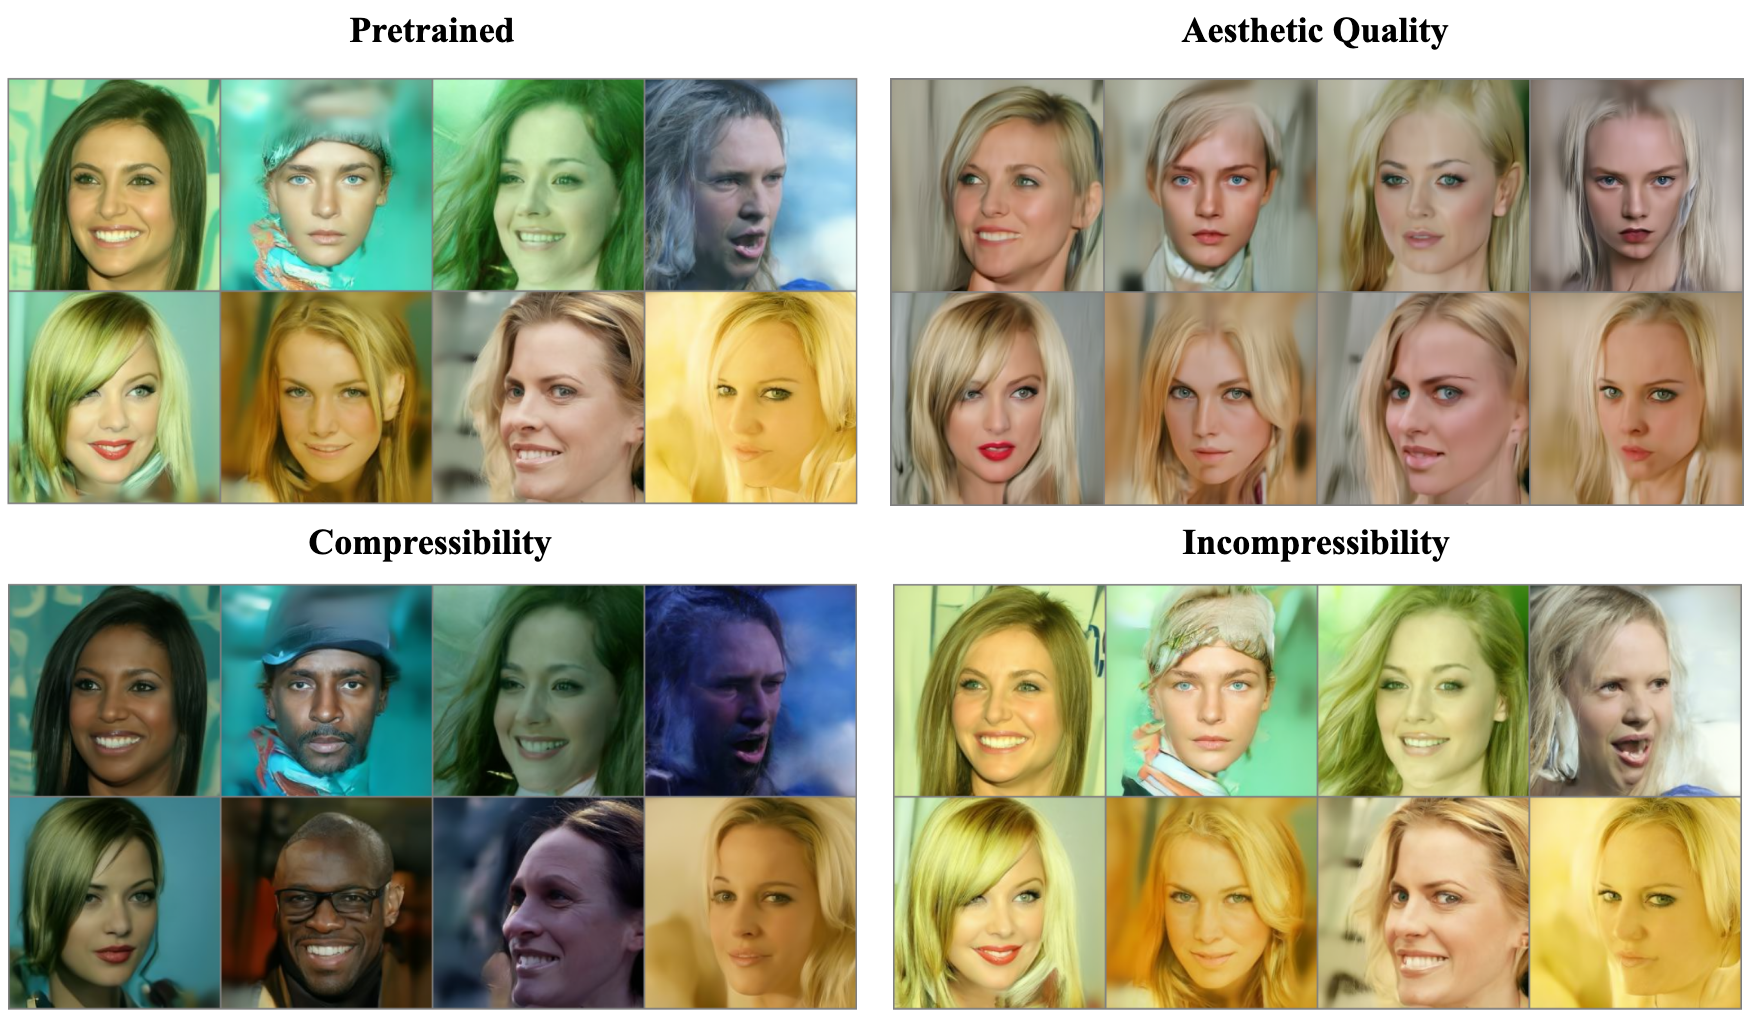
\includegraphics[scale=0.72]{img/results/visual-comparison-results-200dpi.png}
  \vspace{-4pt}  % reduce space between caption and figure
    \captionsetup{width=\textwidth} % set the width of the caption
    \caption{\textbf{DDPO samples vs pretrained samples.} Qualitative depiction of the effects of RL finetuning on different reward functions.}
    \label{fig:visual-comparison-ddpo}
\end{figure}


\section{Discussion \& Limitations}

\lipsum[1]

\lipsum[4]

